\documentclass[../main.tex]{subfiles}

\begin{document}

\section{Introduction}

After completing one CTF each of the HackTheBox (HTB) platform. For this project, each of us will create a Capture the Flag exercise. What we will include in our CTF will depend on what we have learnt on HTB. 

\subsection{HackTheBox}

HackTheBox is a website that's hosts Capture the Flag style exercises. A Capture the Flag is a virtual machine that has one or more vulnerabilities in its systems. The exercise is trying to find and exploit these vulnerabilities to gain (root) access. To be able to do these exercises we first need to 'hack' into the HackTheBox platform as seen below.

\begin{center}
  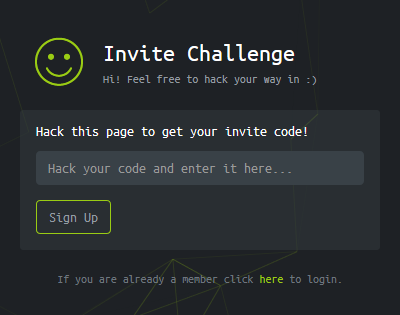
\includegraphics[width=0.5\linewidth]{images/hackthebox_login.png}
\end{center}
 
\subsubsection{Hacking HackTheBox}

As seen above, to gain access to HackTheBox, we need to acquire an invite code. We can easily access a hint to get us started below:

\begin{center}
  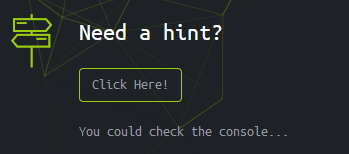
\includegraphics[width=0.5\linewidth]{images/hackthebox_hint.png}
\end{center}

As the hint says, let's look at the console by pressing F12 in Firefox. The first thing we see here is a message telling us to find a javascript file:

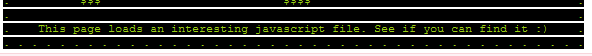
\includegraphics[width=\linewidth]{images/hackthebox_hint2.png}

This file can be found under the 'debugger' tab in the 'js' folder and is called 'inviteapi.min.js'.

\begin{center}
    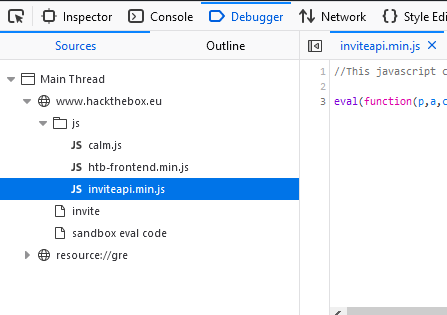
\includegraphics[width=0.5\linewidth]{images/hackthebox_js.png}
\end{center}

Since this is a minified javascipt file (because of the .min.js), there is one line of code in the file. If we copy this file into the 'console' tab and add replace the eval() function with a value assignment (eval(function()) => output = function()) we get an output.

\begin{center}
    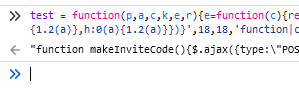
\includegraphics[width=0.5\linewidth]{images/hackthebox_js2.png}
\end{center}

We got a new function as the output string. There are some wrong escape sequences in this function. Once we clean it up and assign it to a value we get another JS function:

\begin{center}
    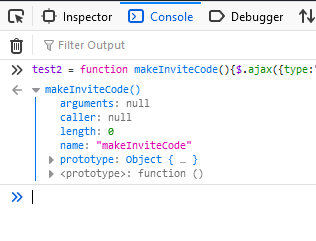
\includegraphics[width=0.5\linewidth]{images/hackthebox_js3.PNG}
\end{center}

\newpage
If we execute this function, we get back this message:

\begin{lstlisting}
{
  "0": 200,
  "success": 1,
  "data": {
    "data": "Va beqre gb trarengr gur vaivgr pbqr, znxr n CBFG erdhrfg gb
    /ncv/vaivgr/trarengr",
    "enctype": "ROT13"
  },
  "hint": "Data is encrypted... We should probably check the encryption 
  type in order to decrypt it..."
}
\end{lstlisting}

This message clearly states the data is encrypted in ROT13. We can use the website \url{https://soumya.dev/decode} to decode from ROT13. If we decode the message, it reads:

\begin{center}
    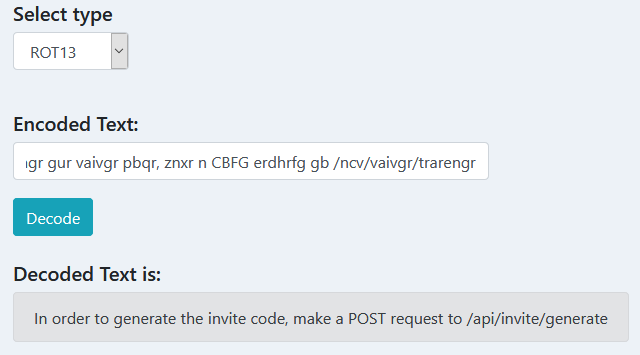
\includegraphics[width=0.75\linewidth]{images/hackthebox_decode.png}
\end{center}

We need to make a POST request to the given path on the HackTheBox website. To do this we use the curl command with the '-X POST' option.

\begin{lstlisting}
$ curl -X POST https://www.hackthebox.eu/api/invite/generate
{"success":1,"data":{"code":"SU1ITVQtQURaRVAtS0tKUEMtTVpWVlEtWFdSSFU=",
"format":"encoded"},"0":200}
\end{lstlisting}

We get back another code that is once again encoded in some way. Inputting this as the access code only returns an error. If we try to decode it with ROT13 like last time, we get back nonsense:

\begin{lstlisting}
FH1VGIDgDHEnEINgF0gXHRZgGIcJIyRgJSqFFSH=
\end{lstlisting}

The site we're using for this decoding has another option available, Base64. Let's try this method of decoding:

\begin{center}
    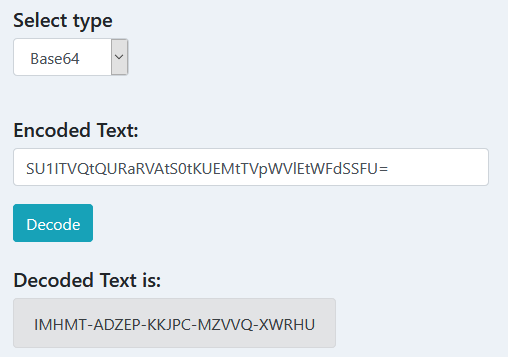
\includegraphics[width=0.75\linewidth]{images/hackthebox_decode2.png}
\end{center}

This code seems to contain a bit more structure, could this be the access code? If we enter it on the website, we do get a congratulations page and are able to register on the site.

\begin{center}
    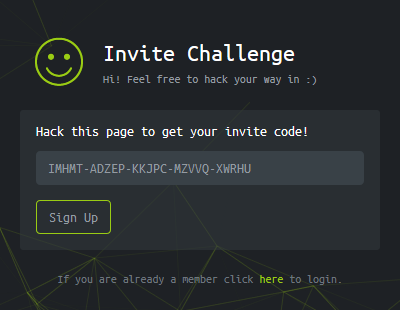
\includegraphics[width=0.75\linewidth]{images/hackthebox_finished.png}
    
\includegraphics[width=0.75\linewidth]{images/hackthebox_finished2.png}
    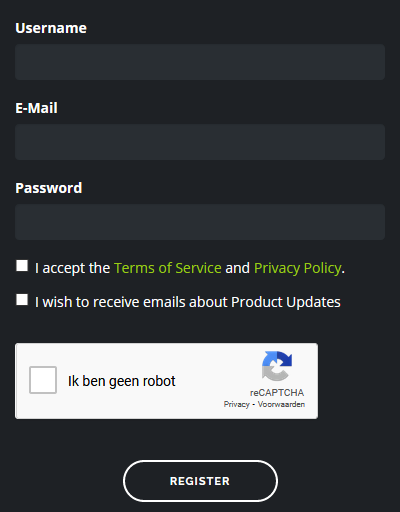
\includegraphics[width=0.75\linewidth]{images/hackthebox_finished3.png}
\end{center}

Now all that remains is to make an account on the website. Everyone in our team has registered an account on the website in this manner. We are ready to get started on our HackTheBox challenges.

\subsection{Getting started with HackTheBox}
Now that we have access to HTB, we're going to see what we need, before we can get started. First of all, we need to download the correct software. What do we need? All you need is a Virtual Machine Management program like VirtualBox or VMware. In our case, we run a virtual Kali Linux machine in VirtualBox.

To get a connection with the lab environment, we need to use OpenVPN, which comes pre-installed on Kali. On the site of Hack The Box you can find a connection pack. Once you've downloaded the .Ovpn connection pack, you can connect to the lab network with the following terminal command:

\begin{lstlisting}
# openvpn example.ovpn
\end{lstlisting}

In the above command, "example.ovpn" should be replaced with the filename or full path of the connection pack. If you're new to HTB, you can try hacking a starting machine which has a full tutorial on how to think and do things. Now we can start our labs.
\end{document}
